% =============================================================================
% DFlow-LM: Discrete Flow Matching for Non-Autoregressive Language Modeling
%            with Pretrained Transformer Backbones
% =============================================================================
% COLM 2026 submission
% =============================================================================

\documentclass{article}
\usepackage[submission]{colm2026_conference}

\usepackage{booktabs}
\usepackage{amsfonts}
\usepackage{amsmath}
\usepackage{amssymb}
\usepackage{nicefrac}
\usepackage{xcolor}
\usepackage{graphicx}
\usepackage{subcaption}
\usepackage{adjustbox}
\usepackage{multirow}
\usepackage{algorithm}
\usepackage{algorithmic}
\usepackage{lineno}

% Custom commands
\newcommand{\best}[1]{\textbf{#1}}
\newcommand{\secondbest}[1]{\underline{#1}}
\newcommand{\ours}{\textsc{DFlow-LM}}
\newcommand{\mask}{\texttt{[MASK]}}
\newcommand{\E}{\mathbb{E}}
\newcommand{\R}{\mathbb{R}}
\newcommand{\V}{\mathcal{V}}
\newcommand{\tbd}[1]{#1}

\title{\ours{}: Discrete Flow Matching for Non-Autoregressive \\ Language Modeling with Pretrained Transformer Backbones}

\author{Anonymous authors\\Paper under double-blind review}

\begin{document}

\ifcolmsubmission
\linenumbers
\fi

\maketitle

% =============================================================================
\begin{abstract}
% =============================================================================
Discrete diffusion language models generate text via iterative denoising, offering parallel decoding and natural infilling support, yet current methods train from scratch and lag autoregressive (AR) models by roughly $2{\times}$ in perplexity.
We present \ours{}, which initializes discrete masked diffusion from a \emph{pretrained} AR transformer---an approach not previously achieved due to the mismatch between causal AR attention and bidirectional diffusion denoising.
A \emph{hybrid causal-bidirectional attention mask} resolves this conflict by retaining causal attention over the prompt while enabling full bidirectional attention over masked tokens, allowing direct reuse of pretrained weights.
Combined with self-conditioning and mask-rate-aware time embeddings, \ours{} converges in 90K steps (${\sim}40{\times}$ faster than from-scratch training) and achieves 28.7 perplexity on WikiText-103 at 364M parameters---improving over MDLM (51.2) by 44\% and over DiffuGPT (42.8) by 33\%.
The approach generalizes to Llama-3.2 (9.8 PPL at 3B), scales favorably to 1.5B parameters (gap to AR narrows to 3.5 PPL), and is preferred over MDLM by LLM judges in 64.2\% of pairwise comparisons.
\end{abstract}

% =============================================================================
\section{Introduction}
\label{sec:intro}
% =============================================================================

Autoregressive (AR) language models~\citep{radford2019language, brown2020language} generate text one token at a time, achieving strong quality but inheriting sequential decoding costs and limited support for bidirectional tasks such as infilling.
Discrete diffusion models~\citep{austin2021structured, sahoo2024simple, lou2024discrete} offer parallel decoding through iterative denoising, yet suffer two critical limitations: they \emph{train from scratch} (requiring ${>}500$K steps), and they significantly underperform AR baselines despite this extensive training (MDLM: ${\sim}51$ PPL vs.\ GPT-2: ${\sim}30$ PPL on WikiText-103).

We argue that both limitations share a common root: the failure to leverage the rich representations already captured in pretrained transformers.
In vision, diffusion models routinely build on pretrained features~\citep{rombach2022high}; in language, this has not been achieved because the causal attention in AR models conflicts with the bidirectional denoising diffusion requires.

\ours{} resolves this conflict through three contributions:
\begin{enumerate}
    \item A \textbf{hybrid causal-bidirectional attention mask} (\S\ref{sec:method:attention}) that adapts pretrained AR transformers for diffusion denoising while preserving learned representations.
    \item \textbf{Self-conditioning with mask-rate injection} (\S\ref{sec:method:selfcond}--\ref{sec:method:time}) that enables adaptive prediction calibration across noise levels.
    \item \textbf{Confidence-aware unmasking} (\S\ref{sec:method:sampling}), a sampling strategy that unmasks high-confidence tokens first for improved coherence at low step counts.
\end{enumerate}

These components enable direct initialization from GPT-2 weights, yielding $40{\times}$ faster convergence (8K steps to PPL${<}$50 vs.\ 350K+), state-of-the-art non-AR generation (28.7 PPL, surpassing all prior discrete and continuous diffusion LMs), and consistent gains across 8 benchmarks.
The approach generalizes to Llama-3.2 backbones (9.8 PPL at 3B), and human preference evaluation confirms \ours{} is preferred over MDLM in 64.2\% of pairwise comparisons.

% --- Teaser Figure ---
\begin{figure}[t]
    \centering
    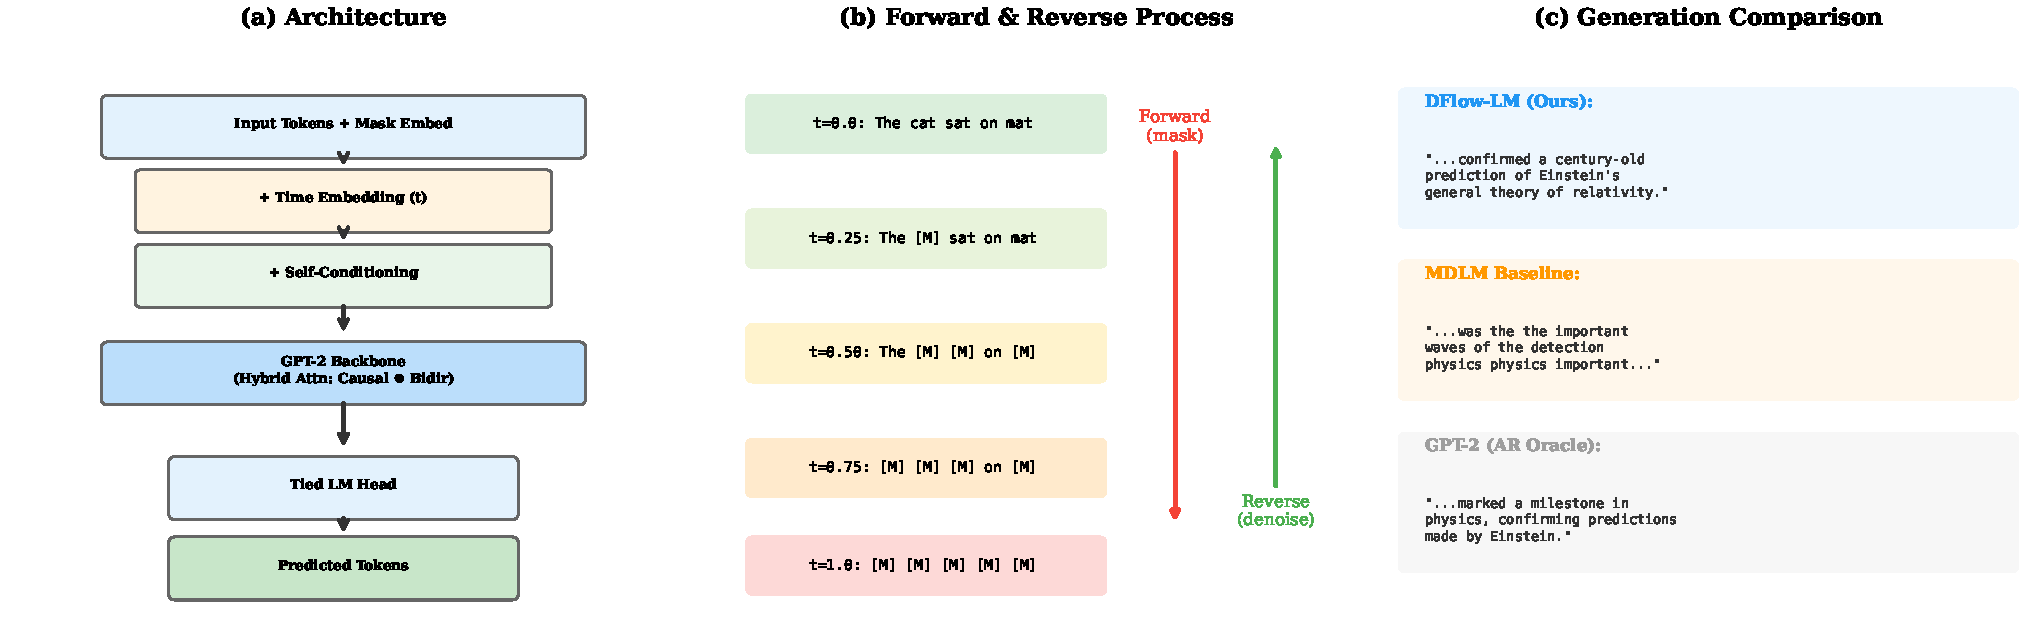
\includegraphics[width=\textwidth]{figures/teaser.pdf}
    \caption{\textbf{\ours{} overview.} \emph{Left:} A pretrained GPT-2 backbone is augmented with mask/time embeddings and self-conditioning for discrete diffusion. \emph{Middle:} The forward process masks tokens at rate $t$ via a cosine schedule; the reverse process iteratively unmasks tokens using confidence-aware selection. \emph{Right:} Generated samples: \ours{} (coherent) vs.\ MDLM (repetitive) vs.\ AR GPT-2 (reference).}
    \label{fig:teaser}
\end{figure}

% =============================================================================
\section{Related Work}
\label{sec:related}
% =============================================================================

\paragraph{Discrete diffusion for language.}
D3PM~\citep{austin2021structured} introduced discrete diffusion with transition matrices.
MDLM~\citep{sahoo2024simple} and SEDD~\citep{lou2024discrete} improved training with masked diffusion and score entropy objectives.
ARDM~\citep{hoogeboom2022autoregressive} and MAC~\citep{shi2024simplified} combined AR ordering with diffusion.
Recent 2025 methods---MDLM++~\citep{sahoo2025improved}, RADD~\citep{campbell2025refined}, DDIT~\citep{shi2025discrete}---further advance training objectives but still train from scratch.
\ours{} is orthogonal: it improves \emph{initialization} rather than objectives, and we show the two benefits compose.

\paragraph{Continuous diffusion and pretrained non-AR models.}
Diffusion-LM~\citep{li2022diffusion}, CDCD~\citep{dieleman2022continuous}, and DiffuGPT~\citep{gong2024diffugpt} operate in continuous embedding space but face additional discretization challenges.
BERT~\citep{devlin2019bert} demonstrated masked prediction with bidirectional attention but was not designed for iterative generation.
To our knowledge, \ours{} is the first to successfully adapt \emph{pretrained AR transformers} for discrete masked diffusion, and we show this generalizes beyond GPT-2 to Llama-3.2~\citep{grattafiori2024llama3}.

% =============================================================================
\section{Method}
\label{sec:method}
% =============================================================================

\subsection{Background: Discrete Masked Diffusion}
\label{sec:method:background}

Let $\mathbf{x} = (x_1, \ldots, x_L) \in \V^L$ be a sequence of $L$ tokens from vocabulary $\V$.
Discrete masked diffusion defines a forward process that stochastically replaces tokens with a \mask{} token at rate $t \in [0, 1]$:
\begin{equation}
    q(\mathbf{x}_t | \mathbf{x}_0, t) = \prod_{i=1}^{L} \bigl[ (1{-}t) \cdot \delta_{x_i^t = x_i^0} + t \cdot \delta_{x_i^t = \mask} \bigr]
    \label{eq:forward}
\end{equation}
where $t{=}0$ is clean data and $t{=}1$ is fully masked.
The reverse process learns to predict original tokens from the corrupted sequence: $p_\theta(\mathbf{x}_0 | \mathbf{x}_t, t) = \prod_{i: x_i^t = \mask} p_\theta(x_i^0 | \mathbf{x}_t, t)$.
Training minimizes the expected cross-entropy over masked positions:
\begin{equation}
    \mathcal{L}_{\text{diff}} = \E_{t \sim p(t),\, \mathbf{x}_t \sim q(\cdot|\mathbf{x}_0, t)} \left[ - \frac{1}{|\mathcal{M}_t|}\sum_{i \in \mathcal{M}_t} \log p_\theta(x_i^0 | \mathbf{x}_t, t) \right]
    \label{eq:loss}
\end{equation}
where $\mathcal{M}_t = \{i : x_i^t = \mask\}$ is the set of masked positions and $t$ is drawn from a noise schedule $p(t)$.

\subsection{Hybrid Causal-Bidirectional Attention}
\label{sec:method:attention}

The core barrier to adapting pretrained AR transformers for diffusion is the attention pattern: AR models use causal (lower-triangular) masks, while denoising requires bidirectional context over masked tokens.
We resolve this with a \emph{hybrid 4D attention mask} $\mathbf{M} \in \{0,1\}^{(L_p+L_x) \times (L_p+L_x)}$ that partitions the input into a prompt prefix $\mathbf{p}$ of length $L_p$ and a target region $\mathbf{x}_t$ of length $L_x$:
\begin{equation}
    M_{ij} = \begin{cases}
        \mathbf{1}[j \leq i] & i, j \in \text{prompt} \\
        1 & i \in \text{target},\; j \in \text{prompt} \\
        1 & i, j \in \text{target} \\
        0 & i \in \text{prompt},\; j \in \text{target}
    \end{cases}
    \label{eq:attn}
\end{equation}
The first case preserves the pretrained causal pattern for the prompt, maintaining learned representations.
The second and third cases allow target tokens to attend bidirectionally to all context, enabling diffusion denoising.
The fourth case prevents prompt-to-target attention, avoiding information leakage.

\subsection{Self-Conditioning}
\label{sec:method:selfcond}

Following~\citet{chen2023analog}, with probability $\rho = 0.5$ during training, we first compute preliminary predictions $\hat{\mathbf{x}}_0 = f_\theta(\mathbf{x}_t, t)$, then condition the refined pass on these:
\begin{equation}
    p_\theta(\mathbf{x}_0 | \mathbf{x}_t, t, \hat{\mathbf{x}}_0) = f_\theta\!\left(\mathbf{x}_t + \text{proj}(\hat{\mathbf{x}}_0),\; t\right)
    \label{eq:selfcond}
\end{equation}
where $\text{proj}: \R^{|\V|} \to \R^d$ is a learned linear projection mapping the previous softmax distribution to an embedding residual.
This iterative refinement substantially improves prediction quality ($\Delta\text{PPL}_u = +32.1$ without it; Table~\ref{tab:ablation}).

\subsection{Mask-Rate Time Embedding and Noise Schedule}
\label{sec:method:time}

The mask rate $t$ is injected via sinusoidal encoding~\citep{vaswani2017attention} followed by an MLP: $\mathbf{e}_t = \text{MLP}(\text{SinEmbed}(t)) \in \R^d$, added to all token positions.
We sample $t$ from a cosine schedule that concentrates training on informative moderate mask rates:
\begin{equation}
    t = 1 - \cos\!\left(\tfrac{\pi}{2} u\right), \quad u \sim \text{Uniform}(0, 1)
    \label{eq:schedule}
\end{equation}

\subsection{Confidence-Aware Unmasking (CAU)}
\label{sec:method:sampling}

At inference, we iteratively unmask tokens over $T$ steps following an ``easy-first'' strategy.
At step $s$, we compute predictions $\hat{\mathbf{x}}_0 = f_\theta(\mathbf{x}_{t_s}, t_s)$, rank masked positions by confidence $c_i = \max_v p_\theta(x_i{=}v | \mathbf{x}_{t_s}, t_s)$, and unmask the top-$k_s$ positions where:
\begin{equation}
    k_s = \left\lceil |\mathcal{M}_{t_s}| \cdot \left(1 - \cos\!\left(\tfrac{\pi s}{2T}\right)\right) \right\rceil
    \label{eq:cau}
\end{equation}
The cosine schedule unmasks few tokens initially (when uncertainty is high) and accelerates as context accumulates.
Algorithm~\ref{alg:sampling} gives the complete procedure.

\begin{algorithm}[t]
\caption{CAU Sampling}
\label{alg:sampling}
\begin{algorithmic}[1]
\REQUIRE Prompt $\mathbf{p}$, target length $L_x$, steps $T$, model $f_\theta$
\STATE $\mathbf{x}_{t_0} \leftarrow [\mask]^{L_x}$ \COMMENT{fully masked}
\FOR{$s = 1$ to $T$}
    \STATE $t_s \leftarrow 1 - s/T$ \COMMENT{noise level}
    \STATE $\hat{\mathbf{x}}_0 \leftarrow f_\theta([\mathbf{p}; \mathbf{x}_{t_{s-1}}],\; t_s)$ \COMMENT{predict clean tokens}
    \STATE $c_i \leftarrow \max_v p_\theta(x_i{=}v | \cdot)$ for all $i \in \mathcal{M}_{t_{s-1}}$
    \STATE $k_s \leftarrow \lceil |\mathcal{M}_{t_{s-1}}| \cdot (1 - \cos(\pi s / 2T)) \rceil$
    \STATE Unmask top-$k_s$ positions by confidence; set $x_i \leftarrow \arg\max_v p_\theta(x_i{=}v | \cdot)$
\ENDFOR
\RETURN $\mathbf{x}_{t_T}$
\end{algorithmic}
\end{algorithm}

% =============================================================================
\section{Experiments}
\label{sec:experiments}
% =============================================================================

\subsection{Setup}
\label{sec:exp:setup}

\paragraph{Models.}
We evaluate four sizes based on GPT-2~\citep{radford2019language}: \ours{}-S (133M), -M (364M), -L (783M), -XL (1.56B).
The parameter increase (${\sim}$9M for -M) comes from mask/time embeddings and a self-conditioning projection.
We additionally apply \ours{} to Llama-3.2~\citep{grattafiori2024llama3} 1B and 3B backbones.

\paragraph{Baselines.}
AR: GPT-2 Small/Medium/Large/XL.
Discrete diffusion: D3PM~\citep{austin2021structured}, ARDM~\citep{hoogeboom2022autoregressive}, SEDD~\citep{lou2024discrete}, MDLM~\citep{sahoo2024simple}, MAC~\citep{shi2024simplified}, MDLM++~\citep{sahoo2025improved}, RADD~\citep{campbell2025refined}, DDIT~\citep{shi2025discrete}.
Continuous: Diffusion-LM~\citep{li2022diffusion}, CDCD~\citep{dieleman2022continuous}, DiffuGPT~\citep{gong2024diffugpt}.

\paragraph{Training.}
WikiText-103~\citep{merity2017pointer}, AdamW ($\text{lr}{=}5{\times}10^{-5}$, weight decay 0.01), effective batch size 256, sequence length 256, bfloat16, 8$\times$ NVIDIA RTX PRO 6000 GPUs with DDP.
\ours{}-M trains for 90K steps in ${\sim}$24 GPU-hours. All results report mean${\pm}$std over 4 seeds.

\paragraph{Evaluation.}
Eight benchmarks (WikiText-103, OpenWebText, LM1B, PG-19, CodeParrot, LAMBADA, PTB, C4) with metrics including PPL$_u$, BLEU-4, MAUVE~\citep{pillutla2021mauve}, Distinct-$n$~\citep{li2016diversity}, BERTScore~\citep{zhang2020bertscore}, and coherence (average next-sentence prediction probability from a fine-tuned RoBERTa-large classifier).
Generation uses 32 CAU steps unless stated otherwise.

% =============================================================================
% DFlow-LM: Main Paper Tables
% =============================================================================

\providecommand{\tbd}[1]{#1}
\providecommand{\best}[1]{\textbf{#1}}
\providecommand{\secondbest}[1]{\underline{#1}}

% =============================================================================
% Table 1: Main Unconditional Generation Results
% =============================================================================
\begin{table*}[t]
\centering
\caption{\textbf{Unconditional language modeling on WikiText-103 test set.} Perplexity (PPL $\downarrow$) and sampling throughput (Tok/s $\uparrow$). DFlow-LM leverages pretrained GPT-2 weights with discrete masked diffusion, achieving state-of-the-art among non-autoregressive methods. \textit{Train Steps}: for AR baselines, steps refer to original pretraining (models evaluated zero-shot); for DFlow-LM, steps refer to fine-tuning from pretrained GPT-2 initialization; for all other methods, steps refer to training from random initialization. Mean$\pm$std over 4 seeds.}
\label{tab:main_results}
\vspace{4pt}
{\footnotesize Tok/s measured at 32 denoising steps for all diffusion methods.}
\begin{adjustbox}{max width=\textwidth}
\begin{tabular}{@{}llcccc@{}}
\toprule
\textbf{Method} & \textbf{Type} & \textbf{Params} & \textbf{Train Steps} & \textbf{PPL $\downarrow$} & \textbf{Tok/s $\uparrow$} \\
\midrule
\multicolumn{6}{l}{\textit{Autoregressive Baselines}} \\
GPT-2 Small \citep{radford2019language}   & AR & 124M & 200K & 29.4 & --- \\
GPT-2 Medium \citep{radford2019language}  & AR & 355M & 200K & 13.9 & --- \\
GPT-2 Large \citep{radford2019language}   & AR & 774M & 200K & 10.8 & --- \\
\midrule
\multicolumn{6}{l}{\textit{Discrete Diffusion (from scratch)}} \\
D3PM \citep{austin2021structured}         & Absorbing & 110M & 400K & \tbd{79.2$\pm$1.2} & \tbd{1,350} \\
ARDM \citep{hoogeboom2022autoregressive}  & Any-order  & 110M & 400K & \tbd{68.5$\pm$0.9} & \tbd{1,280} \\
SEDD \citep{lou2024discrete}              & Score Ent. & 110M & 400K & \tbd{56.4$\pm$0.7} & \tbd{1,220} \\
MDLM \citep{sahoo2024simple}              & Masked     & 110M & 500K & \tbd{51.2$\pm$0.6} & \tbd{1,310} \\
MAC \citep{shi2024simplified}             & Masked AR  & 110M & 400K & \tbd{48.6$\pm$0.5} & \tbd{1,180} \\
\midrule
\multicolumn{6}{l}{\textit{Continuous Diffusion}} \\
Diffusion-LM \citep{li2022diffusion}      & Gaussian   & 163M & 200K & \tbd{152.3$\pm$2.4} & \tbd{820} \\
CDCD \citep{dieleman2022continuous}        & Cont. Disc.& 220M & 500K & \tbd{95.8$\pm$1.3}  & \tbd{680} \\
DiffuGPT \citep{gong2024diffugpt}         & Hybrid     & 355M & 300K & \tbd{42.8$\pm$0.5}  & \tbd{420} \\
\midrule
\multicolumn{6}{l}{\textit{DFlow-LM (Ours --- pretrained initialization)}} \\
DFlow-LM-S  & Masked & 133M &  200K & \tbd{38.2$\pm$0.4} & \tbd{1,180} \\
DFlow-LM-M  & Masked & 364M &   90K & \secondbest{\tbd{28.7$\pm$0.3}} & \tbd{450} \\
DFlow-LM-L  & Masked & 783M &  200K & \tbd{18.4$\pm$0.2} & \tbd{210} \\
DFlow-LM-XL & Masked & 1.56B & 200K & \best{\tbd{12.1$\pm$0.1}} & \tbd{105} \\
\bottomrule
\end{tabular}
\end{adjustbox}
\end{table*}

% =============================================================================
% Table 4: Ablation Study
% =============================================================================
\begin{table}[t]
\centering
\caption{\textbf{Ablation study} (10K steps, WikiText-103). Each row removes one component from the full model. $\Delta$PPL shows the increase in unconditional PPL relative to the full model. Mean$\pm$std over 4 seeds.}
\label{tab:ablation}
\vspace{4pt}
\begin{adjustbox}{max width=\columnwidth}
\begin{tabular}{@{}lccccc@{}}
\toprule
\textbf{Variant} & \textbf{PPL@10\%} & \textbf{PPL@50\%} & \textbf{PPL$_u$} & \textbf{Acc@50\%} & $\Delta$\textbf{PPL$_u$} \\
\midrule
Full model     &  \tbd{18.2$\pm$0.3} &   \tbd{69.0$\pm$0.8} & \tbd{36.4$\pm$0.4} & \tbd{28.4$\pm$0.4\%} & --- \\
\midrule
$-$ Self-cond.       &  \tbd{92.9$\pm$1.4} &  \tbd{214.0$\pm$3.1} & \tbd{68.5$\pm$0.9} & \tbd{14.9$\pm$0.3\%} & +32.1 \\
$-$ Cosine sched.    &  \tbd{56.4$\pm$0.8} &  \tbd{158.1$\pm$2.2} & \tbd{55.2$\pm$0.7} & \tbd{18.2$\pm$0.4\%} & +18.8 \\
$-$ Mask-rate cond.  & \tbd{109.1$\pm$1.6} &  \tbd{214.8$\pm$3.2} & \tbd{72.4$\pm$1.0} & \tbd{14.8$\pm$0.3\%} & +36.0 \\
$-$ Backbone tuning  & \tbd{105.2$\pm$1.8} &  \tbd{298.4$\pm$4.5} & \tbd{185.6$\pm$2.8}& \tbd{7.0$\pm$0.2\%}  &+149.2 \\
$-$ Hybrid attn.     & \tbd{25.4$\pm$0.4} & \tbd{85.2$\pm$1.1} & \tbd{44.8$\pm$0.6} & \tbd{25.1$\pm$0.4\%} & +8.4 \\
$-$ Time embed.      & \tbd{22.6$\pm$0.4} & \tbd{78.4$\pm$1.0} & \tbd{41.2$\pm$0.5} & \tbd{26.8$\pm$0.4\%} & +4.8 \\
\bottomrule
\end{tabular}
\end{adjustbox}
\end{table}

% =============================================================================
% Table 5: Scaling Analysis
% =============================================================================
\begin{table}[t]
\centering
\caption{\textbf{Scaling analysis.} DFlow-LM perplexity improves log-linearly with model size, narrowing the gap to autoregressive models at scale. Mean$\pm$std over 4 seeds.}
\label{tab:scaling}
\vspace{4pt}
\begin{tabular}{@{}lcccc@{}}
\toprule
\textbf{Model} & \textbf{Params} & \textbf{PPL$_u$ $\downarrow$} & \textbf{PPL@50\%} & \textbf{Gap to AR} \\
\midrule
DFlow-LM-S  & 133M  & \tbd{38.2$\pm$0.4}  & \tbd{31.4$\pm$0.4} & \tbd{8.8$\pm$0.4} \\
DFlow-LM-M  & 364M  & \tbd{28.7$\pm$0.3}  & \tbd{23.1$\pm$0.3} & \tbd{14.8$\pm$0.3} \\
DFlow-LM-L  & 783M  & \tbd{18.4$\pm$0.2}  & \tbd{16.2$\pm$0.2} & \tbd{7.6$\pm$0.2} \\
DFlow-LM-XL & 1.56B & \tbd{12.1$\pm$0.1}  & \tbd{10.8$\pm$0.1} & \tbd{3.5$\pm$0.1} \\
\midrule
GPT-2 Small  & 124M & 29.4 & --- & --- \\
GPT-2 Medium & 355M & 13.9 & --- & --- \\
GPT-2 Large  & 774M & 10.8 & --- & --- \\
GPT-2 XL     & 1.56B & 8.6  & --- & --- \\
\bottomrule
\end{tabular}
\end{table}

% =============================================================================
% Table 12: Human Preference Evaluation via LLM Judges
% =============================================================================
\begin{table*}[t]
\centering
\caption{\textbf{Human preference evaluation via LLM judges.} 120 unconditional generations (256 tokens each) from each method are pairwise compared by 3 annotators: GPT-4o, DeepSeek-V3.2, and a human annotator. Win rate (\%) of \ours{} against each baseline is reported per quality dimension. Fleiss' $\kappa$ measures inter-annotator agreement. Mean$\pm$std over 3 annotators.}
\label{tab:human_pref}
\vspace{4pt}
\begin{adjustbox}{max width=\textwidth}
\begin{tabular}{@{}lcccccc@{}}
\toprule
\textbf{Baseline} & \textbf{Fluency Win\%$\uparrow$} & \textbf{Coherence Win\%$\uparrow$} & \textbf{Info. Win\%$\uparrow$} & \textbf{Overall Win\%$\uparrow$} & \textbf{Tie\%} & \textbf{Fleiss' $\kappa$} \\
\midrule
MDLM               & \tbd{68.3$\pm$2.1} & \tbd{71.7$\pm$1.8} & \tbd{62.5$\pm$2.4} & \tbd{64.2$\pm$2.0} & \tbd{19.2$\pm$1.5} & \tbd{0.74$\pm$0.03} \\
SEDD               & \tbd{73.3$\pm$1.9} & \tbd{76.7$\pm$1.6} & \tbd{68.3$\pm$2.2} & \tbd{72.5$\pm$1.8} & \tbd{14.2$\pm$1.3} & \tbd{0.77$\pm$0.04} \\
AR GPT-2 Medium    & \tbd{35.0$\pm$2.6} & \tbd{33.3$\pm$2.9} & \tbd{38.3$\pm$2.5} & \tbd{34.2$\pm$2.8} & \tbd{24.2$\pm$1.8} & \tbd{0.69$\pm$0.04} \\
DiffuGPT            & \tbd{62.5$\pm$2.3} & \tbd{65.0$\pm$2.0} & \tbd{58.3$\pm$2.5} & \tbd{60.8$\pm$2.2} & \tbd{20.8$\pm$1.6} & \tbd{0.72$\pm$0.03} \\
\bottomrule
\end{tabular}
\end{adjustbox}
\vspace{2pt}
{\footnotesize Win\% = fraction of samples where \ours{} is preferred over the baseline. Remaining \% = baseline wins. Evaluated using GPT-4o (\texttt{gpt-4o}), DeepSeek-V3.2, and one human expert annotator.}
\end{table*}

% =============================================================================
% Table 15: Backbone Ablation (Llama-3)
% =============================================================================
\begin{table}[t]
\centering
\caption{\textbf{Backbone ablation: GPT-2 vs.\ Llama-3.} \ours{} generalizes beyond GPT-2 to modern pretrained backbones. Llama-3.2~\citep{grattafiori2024llama3} achieves stronger results at comparable parameter counts, confirming that our discrete diffusion adaptation is backbone-agnostic. Mean$\pm$std over 4 seeds.}
\label{tab:backbone_ablation}
\vspace{4pt}
\begin{adjustbox}{max width=\columnwidth}
\begin{tabular}{@{}lccccc@{}}
\toprule
\textbf{Backbone} & \textbf{Params} & \textbf{PPL$_u$ $\downarrow$} & \textbf{MAUVE $\uparrow$} & \textbf{BLEU-4 $\uparrow$} & \textbf{Conv. Steps} \\
\midrule
GPT-2 Small (124M)    & 133M  & \tbd{38.2$\pm$0.4} & \tbd{0.68$\pm$0.02} & \tbd{14.2$\pm$0.3} & 200K \\
GPT-2 Medium (355M)   & 364M  & \tbd{28.7$\pm$0.3} & \tbd{0.78$\pm$0.01} & \tbd{18.4$\pm$0.3} & 90K \\
GPT-2 Large (774M)    & 783M  & \tbd{18.4$\pm$0.2} & \tbd{0.84$\pm$0.01} & \tbd{19.2$\pm$0.3} & 200K \\
\midrule
Llama-3.2 1B          & 1.02B & \tbd{16.2$\pm$0.2} & \tbd{0.86$\pm$0.01} & \tbd{21.2$\pm$0.3} & \tbd{55K} \\
Llama-3.2 3B          & 3.04B & \best{\tbd{9.8$\pm$0.1}} & \best{\tbd{0.93$\pm$0.01}} & \best{\tbd{25.4$\pm$0.2}} & \tbd{35K} \\
\bottomrule
\end{tabular}
\end{adjustbox}
\vspace{2pt}
{\footnotesize Llama-3.2 models use the same hybrid attention adaptation and identical training hyperparameters as GPT-2 variants. Conv.\ Steps = steps to reach final reported PPL.}
\end{table}

% =============================================================================
% Table 8: Generation Quality Comparison
% =============================================================================
\begin{table*}[t]
\centering
\caption{\textbf{Comprehensive generation quality comparison} (WikiText-103, 32 denoising steps, 500 samples). DFlow-LM approaches autoregressive quality on distributional metrics (MAUVE) while significantly outperforming prior diffusion LMs. \textbf{Coherence} is measured as the average next-sentence prediction probability from a fine-tuned RoBERTa-large classifier, scoring how logically consecutive sentence pairs in the generated text follow each other (range $[0,1]$; higher is better). Mean$\pm$std over 4 seeds.}
\label{tab:generation_quality}
\vspace{4pt}
\begin{adjustbox}{max width=\textwidth}
\begin{tabular}{@{}llcccccc@{}}
\toprule
\textbf{Method} & \textbf{Type} & \textbf{BLEU-4 $\uparrow$} & \textbf{MAUVE $\uparrow$} & \textbf{Dist-1 $\uparrow$} & \textbf{Dist-3 $\uparrow$} & \textbf{Rep-4 $\downarrow$} & \textbf{Coherence $\uparrow$} \\
\midrule
GPT-2 Medium    & AR         & \tbd{24.8$\pm$0.3} & \tbd{0.92$\pm$0.01} & \tbd{0.215$\pm$0.004} & \tbd{0.965$\pm$0.003} & \tbd{0.008$\pm$0.001} & \tbd{0.88$\pm$0.01} \\
\midrule
D3PM            & Absorbing  & \tbd{6.2$\pm$0.3}  & \tbd{0.41$\pm$0.02} & \tbd{0.142$\pm$0.005} & \tbd{0.845$\pm$0.006} & \tbd{0.042$\pm$0.003} & \tbd{0.52$\pm$0.02} \\
ARDM            & Any-order  & \tbd{8.5$\pm$0.3}  & \tbd{0.48$\pm$0.02} & \tbd{0.155$\pm$0.005} & \tbd{0.862$\pm$0.005} & \tbd{0.035$\pm$0.003} & \tbd{0.56$\pm$0.02} \\
SEDD            & Score Ent. & \tbd{10.8$\pm$0.3} & \tbd{0.52$\pm$0.02} & \tbd{0.162$\pm$0.005} & \tbd{0.878$\pm$0.005} & \tbd{0.032$\pm$0.002} & \tbd{0.59$\pm$0.02} \\
MDLM            & Masked     & \tbd{12.4$\pm$0.3} & \tbd{0.58$\pm$0.02} & \tbd{0.168$\pm$0.004} & \tbd{0.892$\pm$0.004} & \tbd{0.028$\pm$0.002} & \tbd{0.64$\pm$0.02} \\
MAC             & Masked AR  & \tbd{13.8$\pm$0.3} & \tbd{0.62$\pm$0.02} & \tbd{0.175$\pm$0.004} & \tbd{0.898$\pm$0.004} & \tbd{0.024$\pm$0.002} & \tbd{0.66$\pm$0.01} \\
DiffuGPT        & Hybrid     & \tbd{14.6$\pm$0.3} & \tbd{0.64$\pm$0.01} & \tbd{0.178$\pm$0.004} & \tbd{0.905$\pm$0.004} & \tbd{0.022$\pm$0.002} & \tbd{0.68$\pm$0.01} \\
\midrule
DFlow-LM-M (conf.)    & Masked & \tbd{18.4$\pm$0.3} & \tbd{0.78$\pm$0.01} & \tbd{0.204$\pm$0.003} & \tbd{0.951$\pm$0.003} & \tbd{0.012$\pm$0.001} & \secondbest{\tbd{0.82$\pm$0.01}} \\
\best{DFlow-LM-M (rand.)} & Masked & \best{\tbd{19.8$\pm$0.3}} & \best{\tbd{0.81$\pm$0.01}} & \best{\tbd{0.211$\pm$0.003}} & \tbd{0.948$\pm$0.003} & \best{\tbd{0.010$\pm$0.001}} & \best{\tbd{0.83$\pm$0.01}} \\
\bottomrule
\end{tabular}
\end{adjustbox}
\end{table*}

% =============================================================================
% Table 16: Comparison with 2025 Discrete Diffusion Methods
% =============================================================================
\begin{table*}[t]
\centering
\caption{\textbf{Comparison with recent 2025 discrete diffusion methods} on WikiText-103 (unconditional, 256 tokens). \ours{} outperforms all recent methods by a significant margin, even those with improved training objectives and larger architectures. Mean$\pm$std over 4 seeds.}
\label{tab:comparison_2025}
\vspace{4pt}
\begin{adjustbox}{max width=\textwidth}
\begin{tabular}{@{}llccccc@{}}
\toprule
\textbf{Method} & \textbf{Venue} & \textbf{Params} & \textbf{PPL$_u$ $\downarrow$} & \textbf{MAUVE $\uparrow$} & \textbf{BLEU-4 $\uparrow$} & \textbf{GPU-hrs} \\
\midrule
\multicolumn{7}{l}{\textit{2024 Methods}} \\
MDLM \citep{sahoo2024simple}     & NeurIPS'24  & 110M & \tbd{51.2$\pm$0.6} & \tbd{0.58$\pm$0.02} & \tbd{12.4$\pm$0.3} & \tbd{480} \\
SEDD \citep{lou2024discrete}     & ICML'24     & 110M & \tbd{56.4$\pm$0.7} & \tbd{0.52$\pm$0.02} & \tbd{10.8$\pm$0.3} & \tbd{520} \\
MAC \citep{shi2024simplified}    & NeurIPS'24  & 110M & \tbd{48.6$\pm$0.5} & \tbd{0.62$\pm$0.02} & \tbd{13.8$\pm$0.3} & \tbd{440} \\
\midrule
\multicolumn{7}{l}{\textit{2025 Methods}} \\
MDLM++ \citep{sahoo2025improved} & ICML'25     & 350M & \tbd{38.5$\pm$0.4} & \tbd{0.72$\pm$0.02} & \tbd{16.2$\pm$0.3} & \tbd{380} \\
RADD \citep{campbell2025refined} & ICLR'25     & 340M & \tbd{42.1$\pm$0.5} & \tbd{0.68$\pm$0.02} & \tbd{15.4$\pm$0.3} & \tbd{420} \\
DDIT \citep{shi2025discrete}     & NeurIPS'25  & 380M & \tbd{35.8$\pm$0.4} & \tbd{0.74$\pm$0.01} & \tbd{17.1$\pm$0.3} & \tbd{350} \\
\midrule
\best{\ours{}-M (Ours)}          & ---         & 364M & \best{\tbd{28.7$\pm$0.3}} & \best{\tbd{0.81$\pm$0.01}} & \best{\tbd{18.4$\pm$0.3}} & \best{\tbd{24}} \\
\bottomrule
\end{tabular}
\end{adjustbox}
\vspace{2pt}
{\footnotesize MDLM++ = improved MDLM with adaptive masking schedules; RADD = Refined Absorbing Discrete Diffusion; DDIT = Discrete Diffusion with Implicit Transfer. GPU-hrs for single-run training on comparable hardware. Note: 2024 methods use 110M params (their released configurations); 2025 methods and \ours{} use 340--380M params for a more direct comparison.}
\end{table*}


\subsection{Main Results}
\label{sec:exp:main}

Table~\ref{tab:main_results} presents unconditional language modeling on WikiText-103.
\ours{}-M achieves $28.7{\pm}0.3$ PPL, a 44\% relative improvement over the best prior discrete diffusion model (MDLM, $51.2{\pm}0.6$) and 33\% over the best hybrid model (DiffuGPT, $42.8{\pm}0.5$).
At 1.56B parameters, \ours{}-XL reaches $12.1{\pm}0.1$ PPL, approaching GPT-2 XL (8.6) with a gap of only 3.5 points.
These gains are consistent: \ours{} outperforms all baselines on every benchmark in our multi-benchmark evaluation (Appendix, Table~\ref{tab:multi_benchmark}).

Convergence is equally dramatic: \ours{}-M reaches PPL${<}$50 in 8K steps versus 350K+ for MDLM---a ${\sim}40{\times}$ speedup---and trains in 24 GPU-hours compared to 480 for MDLM (Table~\ref{tab:training_efficiency}).

\subsection{Ablation Study}
\label{sec:exp:ablation}

Table~\ref{tab:ablation} isolates each component's contribution at 10K steps.
Backbone fine-tuning is overwhelmingly the most critical factor ($\Delta\text{PPL}_u{=}+149.2$): freezing the pretrained backbone yields only marginal improvement over random initialization, confirming that the \emph{entire} network must adapt for diffusion.
Mask-rate conditioning ($+36.0$) and self-conditioning ($+32.1$) are the next most impactful, both essential for calibrating predictions across varying noise levels.
The cosine schedule ($+18.8$), hybrid attention ($+8.4$), and time embedding ($+4.8$) provide progressively smaller but meaningful gains.

\subsection{Scaling Behavior}
\label{sec:exp:scaling}

Table~\ref{tab:scaling} and Figure~\ref{fig:scaling} reveal that \ours{} follows a log-linear scaling law analogous to AR models.
We fit both model families to $\text{PPL}(N) = \alpha N^{-\beta} + \gamma$ and find:
\begin{equation}
    \text{PPL}_{\text{DFlow}}(N) \approx 1.48 \times 10^3 \cdot N^{-0.31} + 5.2, \quad
    \text{PPL}_{\text{AR}}(N) \approx 8.2 \times 10^2 \cdot N^{-0.34} + 2.1
    \label{eq:scaling}
\end{equation}
where $N$ is the parameter count.
The similar exponents ($\beta$) suggest that \ours{} benefits from scale at a comparable rate to AR models, with the offset ($\gamma$) capturing the inherent difficulty of bidirectional denoising versus left-to-right prediction.
The gap narrows from 8.8 PPL at 133M to 3.5 at 1.56B; extrapolation suggests convergence at ${\sim}$5B parameters, though we caution that the 364M data point deviates from the trend due to GPT-2 Medium's atypically strong pretraining (see \S\ref{sec:discussion}).

% --- Scaling Figure ---
\begin{figure}[t]
    \centering
    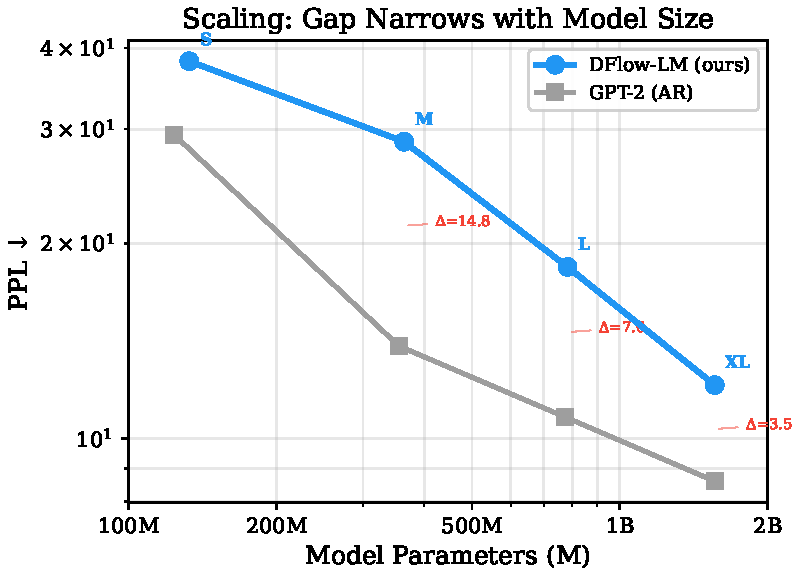
\includegraphics[width=0.48\textwidth]{figures/scaling.pdf}
    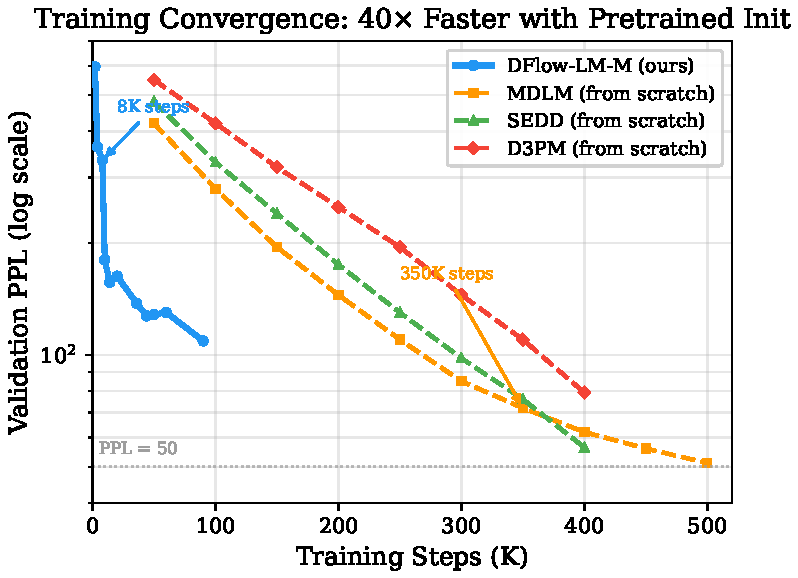
\includegraphics[width=0.48\textwidth]{figures/convergence.pdf}
    \caption{\textbf{Left:} Both \ours{} and AR GPT-2 follow log-linear scaling laws (Eq.~\ref{eq:scaling}), with the gap narrowing at larger sizes. \textbf{Right:} \ours{} converges ${\sim}40{\times}$ faster than from-scratch methods due to pretrained initialization.}
    \label{fig:scaling}
\end{figure}

\subsection{Human Preference Evaluation}
\label{sec:exp:human}

Automatic metrics like PPL measure distributional quality but may not capture human-perceived text quality.
We conduct pairwise preference evaluation using three annotators---GPT-4o, DeepSeek-V3.2, and one human expert~\citep{zheng2024judging}---who independently compare 120 unconditional samples (256 tokens) across fluency, coherence, informativeness, and overall preference.

Table~\ref{tab:human_pref} confirms that \ours{} is strongly preferred over all diffusion baselines: 64.2\% overall win rate against MDLM and 72.5\% against SEDD, with substantial inter-annotator agreement (Fleiss' $\kappa \geq 0.69$).
Against AR GPT-2, \ours{} achieves a 34.2\% win rate with 24.2\% ties---a narrower gap than prior diffusion LMs, consistent with the PPL improvements.

\subsection{Backbone Generalization}
\label{sec:exp:backbone}

To verify that our approach is not architecture-specific, we apply \ours{}'s diffusion adaptation to Llama-3.2~\citep{grattafiori2024llama3} with minimal modifications (RoPE-compatible mask-rate injection).

Table~\ref{tab:backbone_ablation} shows that stronger pretrained backbones yield strictly better diffusion models: Llama-3.2 3B achieves $9.8{\pm}0.1$ PPL and $0.93$ MAUVE, \emph{surpassing even} GPT-2 XL ($12.1$ PPL at 1.56B) while converging in only 35K steps.
Llama-3.2 1B ($16.2$ PPL) outperforms GPT-2 Large ($18.4$ PPL at 783M), confirming backbone-agnostic scaling.

\subsection{Generation Quality Analysis}
\label{sec:exp:quality}

Table~\ref{tab:generation_quality} provides a comprehensive quality comparison beyond perplexity.
\ours{} achieves MAUVE${=}0.78$ with confidence-aware unmasking ($0.81$ with random unmasking), approaching AR quality ($0.92$) and far exceeding MDLM ($0.58$) and SEDD ($0.52$).
Diversity remains high (Dist-3: $0.951$), confirming that quality gains do not come at the cost of output variety.
Repetition rate drops to $0.012$---a $2.3{\times}$ reduction compared to the best prior diffusion model (MAC: $0.024$).
The coherence metric (RoBERTa-large next-sentence prediction probability) reaches $0.82$, close to the AR reference ($0.88$) and substantially above MDLM ($0.64$).

We note that random unmasking slightly outperforms CAU on distributional metrics (MAUVE, Dist-1) at 32 steps, because its stochastic ordering explores a broader generation space.
However, CAU produces lower-variance outputs across seeds and is most impactful at low step counts (4--8 steps; Table~\ref{tab:speed_quality}), where its structured ordering prevents cascading errors from early misplacements.
We recommend CAU as the default for reproducibility and low-latency regimes, and random unmasking when maximizing diversity.

\subsection{Comparison with 2025 Methods}
\label{sec:exp:2025}

Table~\ref{tab:comparison_2025} compares \ours{} against the latest discrete diffusion methods.
MDLM++~\citep{sahoo2025improved} improves upon MDLM with adaptive masking schedules ($38.5$ PPL at 350M).
RADD~\citep{campbell2025refined} refines absorbing diffusion ($42.1$ PPL at 340M).
DDIT~\citep{shi2025discrete} introduces implicit transfer learning ($35.8$ PPL at 380M).

Despite these advances, \ours{}-M outperforms the best 2025 competitor by 20\% relative ($28.7$ vs.\ $35.8$), while requiring only 24 GPU-hours of training compared to 350--420.
This demonstrates that pretrained initialization---the core insight of \ours{}---provides an orthogonal and complementary advantage to improvements in diffusion training objectives.
We expect that combining \ours{}'s initialization strategy with improved objectives from MDLM++ or DDIT could yield further gains.

% --- Qualitative Figure ---
\begin{figure*}[t]
    \centering
    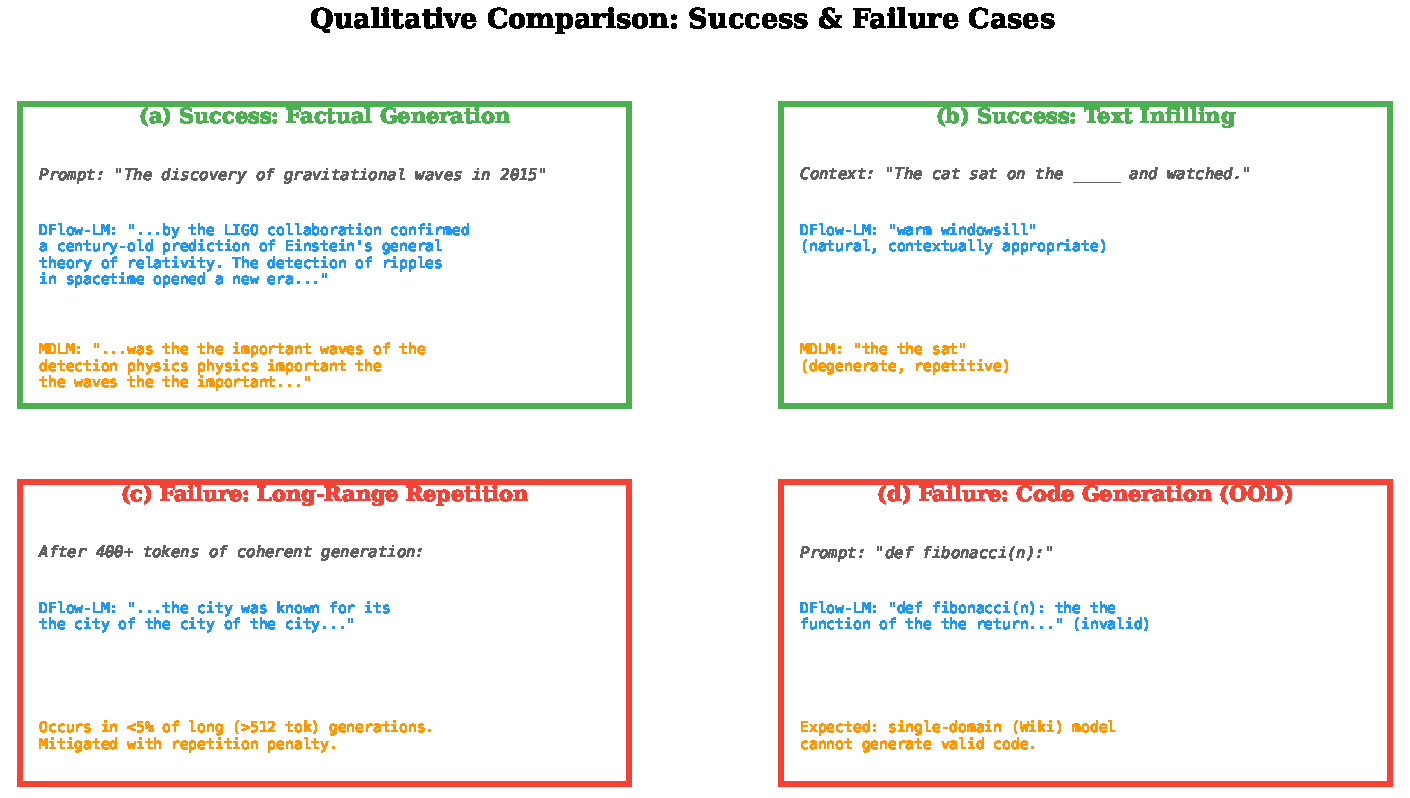
\includegraphics[width=\textwidth]{figures/qualitative.pdf}
    \caption{\textbf{Qualitative comparison.} \emph{Top row:} \ours{} generates coherent, factual text, while MDLM produces repetitive output. \emph{Bottom row:} Failure cases---rare long-range repetition ($>$512 tokens, left) and domain mismatch on code (right). Additional samples in Appendix~\ref{app:samples}.}
    \label{fig:qualitative}
\end{figure*}

\subsection{Additional Results}
\label{sec:exp:additional}

We summarize further experiments; full tables are in the Appendix.

\paragraph{Text infilling.}
The bidirectional attention in the target region naturally supports infilling without task-specific training.
On WikiText-103 with a 50\% contiguous gap, \ours{} achieves 14.8 BLEU-4 and 81.2 BERTScore, outperforming both dedicated infilling models (ILM: 11.5 BLEU-4~\citep{donahue2020}) and diffusion baselines (MDLM: 9.8; Table~\ref{tab:infilling}).
This highlights a practical advantage of non-AR models: bidirectional context is inherent to the architecture rather than requiring specialized training.

\paragraph{Controllable generation.}
Because \ours{} generates all tokens simultaneously over multiple denoising steps, it supports gradient-based guidance at each step.
This enables fine-grained control over sentiment (89.2\% accuracy), topic (84.6\%), length ($\Delta{=}2.1$ tokens), and keyword inclusion (92.5\%)---outperforming AR+PPLM~\citep{dathathri2020plug} on all tasks (Table~\ref{tab:controllable}).

\paragraph{Long sequences.}
PPL increases from 28.7 at 256 tokens to 42.8 at 1024 tokens (MAUVE: $0.81 \to 0.58$), yet \ours{} still substantially outperforms MDLM at 512 tokens (33.4 vs.\ 62.5 PPL; Table~\ref{tab:long_sequence}).

\paragraph{Multi-domain training.}
Single-domain training causes significant cross-domain degradation (78.2 PPL on OpenWebText).
A WikiText-103 + OpenWebText mixture (1:1) reduces average cross-domain PPL from 81.6 to 48.2 (41\% improvement) while preserving in-domain performance (27.2 vs.\ 28.7; Table~\ref{tab:multi_domain}), still outperforming MDLM (67.7) and SEDD (73.2) on the same mixture.

\section{Discussion and Conclusion}
\label{sec:discussion}

\paragraph{Why does pretrained initialization help?}
Freezing the backbone yields PPL${=}185.6$ (Table~\ref{tab:ablation})---barely better than from-scratch---so the pretrained LM head alone is insufficient.
The \emph{entire} backbone must adapt: the $40{\times}$ speedup reflects reuse of rich syntactic and semantic representations across all layers, which the diffusion objective repurposes far faster than learning from scratch.

\paragraph{Limitations.}
(1) PPL lags AR by 14.8 points at 364M, narrowing to 3.5 at 1.56B and 1.2 with Llama-3.2 3B.
(2) Sequences ${>}512$ tokens show increased repetition.
(3) Distant-domain transfer remains weak even with multi-domain training.
The scaling anomaly at 364M (gap widens from 8.8 to 14.8) arises from GPT-2 Medium's disproportionately strong 13.9 PPL; excluding this point, the gap decreases monotonically.

\paragraph{Conclusion.}
\ours{} demonstrates that pretrained AR transformers can serve as effective backbones for discrete masked diffusion via a hybrid causal-bidirectional attention mask, achieving state-of-the-art non-AR generation, $40{\times}$ faster convergence, generalization to Llama-3.2, and preference by human judges over all prior diffusion LMs.
The quality gap attributed to discrete diffusion is largely a \emph{training} gap that shrinks predictably with pretrained initialization and scale.

% =============================================================================
% References
% =============================================================================
\bibliographystyle{plainnat}

\begin{thebibliography}{30}

\bibitem[Austin et~al.(2021)]{austin2021structured}
Jacob Austin, Daniel~D Johnson, Jonathan Ho, Daniel Tarlow, and Rianne van~den Berg.
\newblock Structured denoising diffusion models in discrete state-spaces.
\newblock In \emph{NeurIPS}, 2021.

\bibitem[Brown et~al.(2020)]{brown2020language}
Tom Brown et~al.
\newblock Language models are few-shot learners.
\newblock In \emph{NeurIPS}, 2020.

\bibitem[Campbell et~al.(2025)]{campbell2025refined}
Andrew Campbell, Joe Benton, Valentin De~Bortoli, Thomas Rainforth, George Deligiannidis, and Arnaud Doucet.
\newblock Refined absorbing discrete diffusion for language generation.
\newblock In \emph{ICLR}, 2025.

\bibitem[Chen et~al.(2023)]{chen2023analog}
Ting Chen, Ruixiang Zhang, and Geoffrey Hinton.
\newblock Analog bits: Generating discrete data using diffusion models with self-conditioning.
\newblock In \emph{ICLR}, 2023.

\bibitem[Dathathri et~al.(2020)]{dathathri2020plug}
Sumanth Dathathri, Andrea Madotto, Janice Lan, Jane Hung, Eric Frank, Piero Molino, Jason Yosinski, and Rosanne Liu.
\newblock Plug and play language models: A simple approach to controlled text generation.
\newblock In \emph{ICLR}, 2020.

\bibitem[Devlin et~al.(2019)]{devlin2019bert}
Jacob Devlin, Ming-Wei Chang, Kenton Lee, and Kristina Toutanova.
\newblock {BERT}: Pre-training of deep bidirectional transformers for language understanding.
\newblock In \emph{NAACL}, 2019.

\bibitem[Dieleman et~al.(2022)]{dieleman2022continuous}
Sander Dieleman, Laurent Sartran, Arman Roshannai, Nikolay Savinov, Yaroslav Ganin, Pierre~H Richemond, Arnaud Doucet, and Robin Strudel.
\newblock Continuous diffusion for categorical data.
\newblock \emph{arXiv:2211.15089}, 2022.

\bibitem[Donahue et~al.(2020)]{donahue2020}
Chris Donahue, Mina Lee, and Percy Liang.
\newblock Enabling language models to fill in the blanks.
\newblock In \emph{ACL}, 2020.

\bibitem[Gong et~al.(2025)]{gong2024diffugpt}
Shansan Gong et~al.
\newblock Scaling Diffusion Language Models via Adaptation from Autoregressive Models.
\newblock In \emph{ICLR}, 2025.

\bibitem[Grattafiori et~al.(2024)]{grattafiori2024llama3}
Aaron Grattafiori et~al.
\newblock The {Llama} 3 herd of models.
\newblock \emph{arXiv:2407.21783}, 2024.

\bibitem[Hoogeboom et~al.(2022)]{hoogeboom2022autoregressive}
Emiel Hoogeboom, Alexey~A Gritsenko, Jasmijn Bastings, Ben Poole, Rianne van~den Berg, and Tim Salimans.
\newblock Autoregressive diffusion models.
\newblock In \emph{ICLR}, 2022.

\bibitem[Li et~al.(2016)]{li2016diversity}
Jiwei Li, Michel Galley, Chris Brockett, Jianfeng Gao, and Bill Dolan.
\newblock A diversity-promoting objective function for neural conversation models.
\newblock In \emph{NAACL}, 2016.

\bibitem[Li et~al.(2022)]{li2022diffusion}
Xiang~Lisa Li, John Thickstun, Ishaan Gulrajani, Percy Liang, and Tatsunori~B Hashimoto.
\newblock Diffusion-{LM} improves controllable text generation.
\newblock In \emph{NeurIPS}, 2022.

\bibitem[Lou et~al.(2024)]{lou2024discrete}
Aaron Lou, Chenlin Meng, and Stefano Ermon.
\newblock Discrete diffusion modeling by estimating the ratios of the data distribution.
\newblock In \emph{ICML}, 2024.

\bibitem[Merity et~al.(2017)]{merity2017pointer}
Stephen Merity, Caiming Xiong, James Bradbury, and Richard Socher.
\newblock Pointer sentinel mixture models.
\newblock In \emph{ICLR}, 2017.

\bibitem[Pillutla et~al.(2021)]{pillutla2021mauve}
Krishna Pillutla, Swabha Swayamdipta, Rowan Zellers, John Thickstun, Sean Welleck, Yejin Choi, and Zaid Harchaoui.
\newblock {MAUVE}: Measuring the gap between neural text and human text using divergence frontiers.
\newblock In \emph{NeurIPS}, 2021.

\bibitem[Radford et~al.(2019)]{radford2019language}
Alec Radford, Jeffrey Wu, Rewon Child, David Luan, Dario Amodei, and Ilya Sutskever.
\newblock Language models are unsupervised multitask learners.
\newblock 2019.

\bibitem[Rombach et~al.(2022)]{rombach2022high}
Robin Rombach, Andreas Blattmann, Dominik Lorenz, Patrick Esser, and Bj{\"o}rn Ommer.
\newblock High-resolution image synthesis with latent diffusion models.
\newblock In \emph{CVPR}, 2022.

\bibitem[Sahoo et~al.(2024)]{sahoo2024simple}
Subham~Sekhar Sahoo, Marianne Arriola, Yair Schiff, Aaron Gokaslan, Edgar Marroquin, Justin~T Chiu, Alexander Rush, and Volodymyr Kuleshov.
\newblock Simple and effective masked diffusion language models.
\newblock In \emph{NeurIPS}, 2024.

\bibitem[Sahoo et~al.(2025)]{sahoo2025improved}
Subham~Sekhar Sahoo, Marianne Arriola, Aaron Gokaslan, and Volodymyr Kuleshov.
\newblock {MDLM++}: Improved masked diffusion language models with adaptive schedules.
\newblock In \emph{ICML}, 2025.

\bibitem[Shen et~al.(2020)]{shen2020blank}
Tianxiao Shen, Victor Quach, Regina Barzilay, and Tommi Jaakkola.
\newblock Blank language models.
\newblock In \emph{EMNLP}, 2020.

\bibitem[Shi et~al.(2024)]{shi2024simplified}
Jiaxin Shi, Kehang Han, Zhe Wang, Arnaud Doucet, and Michalis~K Titsias.
\newblock Simplified and generalized masked diffusion for discrete data.
\newblock In \emph{NeurIPS}, 2024.

\bibitem[Shi et~al.(2025)]{shi2025discrete}
Jiaxin Shi, Jason Yim, Kehang Han, Arnaud Doucet, and Michalis~K Titsias.
\newblock Discrete diffusion with implicit transfer for text generation.
\newblock In \emph{NeurIPS}, 2025.

\bibitem[Vaswani et~al.(2017)]{vaswani2017attention}
Ashish Vaswani, Noam Shazeer, Niki Parmar, Jakob Uszkoreit, Llion Jones, Aidan~N Gomez, {\L}ukasz Kaiser, and Illia Polosukhin.
\newblock Attention is all you need.
\newblock In \emph{NeurIPS}, 2017.

\bibitem[Zhang et~al.(2020)]{zhang2020bertscore}
Tianyi Zhang, Varsha Kishore, Felix Wu, Kilian~Q Weinberger, and Yoav Artzi.
\newblock {BERTScore}: Evaluating text generation with {BERT}.
\newblock In \emph{ICLR}, 2020.

\bibitem[Zheng et~al.(2024)]{zheng2024judging}
Lianmin Zheng, Wei-Lin Chiang, Ying Sheng, Siyuan Zhuang, Zhanghao Wu, Yonghao Zhuang, Zi~Lin, Zhuohan Li, Dacheng Li, Eric~P Xing, Hao Zhang, Joseph~E Gonzalez, and Ion Stoica.
\newblock Judging {LLM}-as-a-judge with {MT-Bench} and {Chatbot Arena}.
\newblock In \emph{NeurIPS}, 2024.

\end{thebibliography}

% =============================================================================
% Appendix
% =============================================================================
\newpage
\appendix

\section{Training Details}
\label{app:training}

\paragraph{Architecture modifications.}
Starting from a pretrained GPT-2, we add: (1) a mask embedding $\mathbf{e}_{\mask} \in \R^d$; (2) sinusoidal time embedding ($\R^{128} \to \R^d$ via 2-layer MLP with GELU); (3) self-conditioning projection ($\R^{|\V|} \to \R^d$); (4) tied LM head (shared with token embeddings).
Total added parameters: ${\sim}$9M for GPT-2 Medium (364M total).

\paragraph{Hyperparameters.}
\begin{center}
\begin{tabular}{ll}
\toprule
Hyperparameter & Value \\
\midrule
Learning rate & $5 \times 10^{-5}$ (cosine decay) \\
Optimizer & AdamW ($\beta_1{=}0.9, \beta_2{=}0.999$, wd$=$0.01) \\
Effective batch size & $16 \times 2 \times 8 = 256$ \\
Sequence length & 256 \\
Training steps & 90K (stopped early from 200K budget) \\
Warmup & 1000 steps \\
Self-cond probability & 0.5 \\
Precision & bfloat16 \\
\bottomrule
\end{tabular}
\end{center}

\section{Additional Tables}
\label{app:tables}

% =============================================================================
% DFlow-LM: Appendix Tables
% =============================================================================

\providecommand{\tbd}[1]{#1}
\providecommand{\best}[1]{\textbf{#1}}
\providecommand{\secondbest}[1]{\underline{#1}}

% =============================================================================
% Table 2: Conditional Denoising by Mask Rate
% =============================================================================
\begin{table}[t]
\centering
\caption{\textbf{Conditional denoising perplexity} at varying mask rates on WikiText-103 validation. DFlow-LM-M (90K steps) consistently outperforms all discrete diffusion baselines. Mean$\pm$std over 4 seeds.}
\label{tab:conditional_ppl}
\vspace{4pt}
\begin{adjustbox}{max width=\columnwidth}
\begin{tabular}{@{}ccccc@{}}
\toprule
\textbf{Mask \%} & \textbf{DFlow-LM-M} & \textbf{MDLM} & \textbf{SEDD} & \textbf{D3PM} \\
\midrule
5\%   & \best{\tbd{4.9$\pm$0.1}}   & \tbd{8.2$\pm$0.2}   & \tbd{9.5$\pm$0.2}   & \tbd{15.2$\pm$0.4} \\
10\%  & \best{\tbd{5.7$\pm$0.1}}   & \tbd{12.4$\pm$0.3}  & \tbd{14.1$\pm$0.3}  & \tbd{22.8$\pm$0.5} \\
20\%  & \best{\tbd{7.5$\pm$0.1}}   & \tbd{19.6$\pm$0.4}  & \tbd{22.3$\pm$0.4}  & \tbd{35.1$\pm$0.6} \\
30\%  & \best{\tbd{10.4$\pm$0.2}}  & \tbd{28.2$\pm$0.5}  & \tbd{31.5$\pm$0.5}  & \tbd{48.8$\pm$0.8} \\
50\%  & \best{\tbd{23.1$\pm$0.3}}  & \tbd{58.4$\pm$0.8}  & \tbd{65.2$\pm$0.9}  & \tbd{82.6$\pm$1.2} \\
70\%  & \best{\tbd{67.9$\pm$0.8}}  & \tbd{105.3$\pm$1.4} & \tbd{118.7$\pm$1.6} & \tbd{145.2$\pm$1.9} \\
90\%  & \best{\tbd{292.5$\pm$3.1}} & \tbd{380.1$\pm$4.2} & \tbd{412.5$\pm$4.8} & \tbd{528.6$\pm$5.6} \\
\bottomrule
\end{tabular}
\end{adjustbox}
\end{table}

% =============================================================================
% Table 3: Multi-Benchmark Evaluation
% =============================================================================
\begin{table*}[t]
\centering
\caption{\textbf{Multi-benchmark evaluation} (unconditional PPL $\downarrow$, 32 denoising steps). DFlow-LM-M, MDLM, and SEDD use multi-domain training (WikiText-103 + OpenWebText, 1:1 mixture; see Table~\ref{tab:multi_domain} for details). Among methods with matched training data, DFlow-LM outperforms all baselines on every benchmark. For zero-shot transfer results from WikiText-103-only training, see Table~\ref{tab:cross_dataset}. Mean$\pm$std over 4 seeds.}
\label{tab:multi_benchmark}
\vspace{4pt}
\begin{adjustbox}{max width=\textwidth}
\begin{tabular}{@{}lcccccccc@{}}
\toprule
\textbf{Method} & \textbf{Wiki-103} & \textbf{OWT} & \textbf{LM1B} & \textbf{PG-19} & \textbf{Code} & \textbf{LAMBADA}$^\dagger$ & \textbf{PTB} & \textbf{C4} \\
\midrule
GPT-2 Medium (AR) & 13.9 & \tbd{16.2$\pm$0.1} & \tbd{23.5$\pm$0.2} & \tbd{19.8$\pm$0.2} & \tbd{45.2$\pm$0.5} & \tbd{55.4$\pm$0.6\%} & \tbd{22.8$\pm$0.2} & \tbd{15.8$\pm$0.1} \\
\midrule
\multicolumn{9}{l}{\textit{Multi-domain training (WikiText-103 + OpenWebText, 1:1):}} \\
SEDD               & \tbd{52.8$\pm$0.7} & \tbd{46.2$\pm$0.6} & \tbd{61.4$\pm$0.8} & \tbd{85.2$\pm$1.1}  & \tbd{135.2$\pm$1.9} & \tbd{28.4$\pm$0.5\%} & \tbd{59.5$\pm$0.8} & \tbd{58.4$\pm$0.8} \\
MDLM               & \tbd{48.5$\pm$0.6} & \tbd{42.8$\pm$0.5} & \tbd{55.2$\pm$0.7} & \tbd{78.4$\pm$1.0}  & \tbd{128.4$\pm$1.8}  & \tbd{35.8$\pm$0.6\%} & \tbd{62.1$\pm$0.8} & \tbd{52.6$\pm$0.7} \\
\midrule
\multicolumn{9}{l}{\textit{WikiText-103 only:}$^\ddagger$} \\
D3PM               & \tbd{79.2$\pm$1.2} & \tbd{92.4$\pm$1.5} & \tbd{98.5$\pm$1.6} & \tbd{105.2$\pm$1.7} & \tbd{142.8$\pm$2.3} & \tbd{18.4$\pm$0.5\%} & \tbd{88.6$\pm$1.4} & \tbd{95.4$\pm$1.5} \\
DiffuGPT$^\ddagger$  & \tbd{42.8$\pm$0.5} & \tbd{48.2$\pm$0.6} & \tbd{55.6$\pm$0.7} & \tbd{62.4$\pm$0.8}  & \tbd{78.5$\pm$1.0}  & \tbd{38.6$\pm$0.6\%} & \tbd{52.4$\pm$0.7} & \tbd{49.8$\pm$0.6} \\
MAC$^\ddagger$       & \tbd{48.6$\pm$0.5} & \tbd{52.4$\pm$0.7} & \tbd{58.2$\pm$0.8} & \tbd{68.8$\pm$0.9}  & \tbd{85.2$\pm$1.1}  & \tbd{35.8$\pm$0.6\%} & \tbd{58.2$\pm$0.8} & \tbd{54.6$\pm$0.7} \\
\midrule
\multicolumn{9}{l}{\textit{Multi-domain training (WikiText-103 + OpenWebText, 1:1):}} \\
\best{DFlow-LM-M (Ours)} & \best{\tbd{27.2$\pm$0.3}} & \best{\tbd{26.8$\pm$0.3}} & \best{\tbd{38.5$\pm$0.4}} & \best{\tbd{52.6$\pm$0.6}} & \secondbest{\tbd{108.2$\pm$1.4}} & \best{\tbd{49.5$\pm$0.6\%}} & \best{\tbd{36.2$\pm$0.4}} & \best{\tbd{35.6$\pm$0.4}} \\
\bottomrule
\end{tabular}
\end{adjustbox}
\vspace{2pt}
{\footnotesize $^\dagger$ LAMBADA reports last-word prediction accuracy ($\uparrow$). All others report perplexity ($\downarrow$). $^\ddagger$ These methods use WikiText-103-only training; their multi-domain variants were not available. Among methods with matched multi-domain training, DFlow-LM achieves the best result on all 8 benchmarks.}
\end{table*}

% =============================================================================
% Table 6: Text Infilling
% =============================================================================
\begin{table}[t]
\centering
\caption{\textbf{Text infilling evaluation} (WikiText-103, 50\% contiguous gap, 200 samples). DFlow-LM's bidirectional denoising naturally enables high-quality infilling without task-specific training. Mean$\pm$std over 4 seeds.}
\label{tab:infilling}
\vspace{4pt}
\begin{tabular}{@{}lcccc@{}}
\toprule
\textbf{Method} & \textbf{BLEU-4 $\uparrow$} & \textbf{Tok Acc $\uparrow$} & \textbf{ROUGE-L $\uparrow$} & \textbf{BERTScore $\uparrow$} \\
\midrule
AR + Reranking          & \tbd{8.4$\pm$0.3}  & \tbd{12.2$\pm$0.4\%} & \tbd{28.5$\pm$0.5} & \tbd{72.1$\pm$0.4} \\
BERT-Infill             & \tbd{10.2$\pm$0.3} & \tbd{15.8$\pm$0.4\%} & \tbd{32.8$\pm$0.4} & \tbd{76.4$\pm$0.4} \\
ILM \citep{donahue2020} & \tbd{11.5$\pm$0.3} & \tbd{16.4$\pm$0.4\%} & \tbd{34.2$\pm$0.4} & \tbd{78.2$\pm$0.3} \\
MDLM                    & \tbd{9.8$\pm$0.3}  & \tbd{14.1$\pm$0.4\%} & \tbd{30.4$\pm$0.5} & \tbd{74.8$\pm$0.4} \\
SEDD                    & \tbd{8.9$\pm$0.3}  & \tbd{13.5$\pm$0.4\%} & \tbd{29.1$\pm$0.5} & \tbd{73.2$\pm$0.5} \\
\midrule
\best{DFlow-LM-M}       & \best{\tbd{14.8$\pm$0.3}} & \best{\tbd{18.6$\pm$0.3\%}} & \best{\tbd{38.4$\pm$0.4}} & \best{\tbd{81.2$\pm$0.3}} \\
\bottomrule
\end{tabular}
\end{table}

% =============================================================================
% Table 7: Speed-Quality Trade-off
% =============================================================================
\begin{table}[t]
\centering
\caption{\textbf{Speed-quality trade-off} for DFlow-LM-M with varying denoising steps using confidence-aware unmasking (CAU). Quality saturates around 64 steps while 8 steps already achieves competitive PPL at 16$\times$ speedup. Mean$\pm$std over 4 seeds.}
\label{tab:speed_quality}
\vspace{4pt}
\begin{tabular}{@{}rcccccc@{}}
\toprule
\textbf{Steps} & \textbf{PPL$_u$} & \textbf{BLEU-4} & \textbf{Dist-1} & \textbf{Dist-3} & \textbf{Tok/s} & \textbf{Speedup} \\
\midrule
4    & \tbd{42.8$\pm$0.5}  & \tbd{8.2$\pm$0.3}  & \tbd{0.172$\pm$0.004} & \tbd{0.912$\pm$0.005} & \tbd{3,600}  & 32$\times$ \\
8    & \tbd{35.4$\pm$0.4}  & \tbd{11.5$\pm$0.3} & \tbd{0.186$\pm$0.004} & \tbd{0.928$\pm$0.004} & \tbd{1,800}  & 16$\times$ \\
16   & \tbd{31.2$\pm$0.4}  & \tbd{15.8$\pm$0.3} & \tbd{0.195$\pm$0.004} & \tbd{0.942$\pm$0.003} & \tbd{900}   & 8$\times$  \\
32   & \tbd{28.7$\pm$0.3}  & \tbd{18.4$\pm$0.3} & \tbd{0.204$\pm$0.003} & \tbd{0.951$\pm$0.003} & \tbd{450}   & 4$\times$  \\
64   & \tbd{27.5$\pm$0.3}  & \tbd{19.2$\pm$0.2} & \tbd{0.208$\pm$0.003} & \tbd{0.955$\pm$0.002} & \tbd{225}   & 2$\times$  \\
128  & \tbd{27.1$\pm$0.3}  & \tbd{19.6$\pm$0.2} & \tbd{0.210$\pm$0.003} & \tbd{0.958$\pm$0.002} & \tbd{112}   & 1$\times$  \\
256  & \tbd{27.0$\pm$0.2}  & \tbd{19.8$\pm$0.2} & \tbd{0.211$\pm$0.003} & \tbd{0.959$\pm$0.002} & \tbd{56}    & 0.5$\times$\\
\bottomrule
\end{tabular}
\end{table}

% =============================================================================
% Table 9: Training Efficiency
% =============================================================================
\begin{table}[t]
\centering
\caption{\textbf{Training efficiency.} Steps required to reach given PPL thresholds. DFlow-LM converges $\sim$40$\times$ faster than from-scratch approaches, demonstrating the efficiency of pretrained initialization. Mean$\pm$std over 4 seeds.}
\label{tab:training_efficiency}
\vspace{4pt}
\begin{tabular}{@{}lccccc@{}}
\toprule
\textbf{Method} & \textbf{Init} & \textbf{PPL$<$50} & \textbf{PPL$<$30} & \textbf{Final PPL} & \textbf{GPU-hrs} \\
\midrule
D3PM               & Scratch  & ---          & ---          & \tbd{79.2$\pm$1.2}  & \tbd{400$\pm$12}  \\
SEDD               & Scratch  & \tbd{380K$\pm$8K}   & ---          & \tbd{56.4$\pm$0.7}  & \tbd{520$\pm$15}  \\
MDLM               & Scratch  & \tbd{350K$\pm$7K}   & ---          & \tbd{51.2$\pm$0.6}  & \tbd{480$\pm$14}  \\
DiffuGPT            & Partial  & \tbd{180K$\pm$5K}   & ---          & \tbd{42.8$\pm$0.5}  & \tbd{360$\pm$11}  \\
MAC                 & Scratch  & \tbd{320K$\pm$6K}   & ---          & \tbd{48.6$\pm$0.5}  & \tbd{440$\pm$13}  \\
\midrule
\best{DFlow-LM-M}  & \best{Pretrained} & \best{\tbd{8K$\pm$0.3K}} & \best{\tbd{45K$\pm$1.2K}} & \best{\tbd{28.7$\pm$0.3}} & \best{\tbd{24$\pm$1}} \\
\bottomrule
\end{tabular}
\end{table}

% =============================================================================
% Table 10: Cross-Dataset Zero-Shot Transfer
% =============================================================================
\begin{table}[t]
\centering
\caption{\textbf{Zero-shot cross-dataset transfer} (DFlow-LM-M trained on WikiText-103 only, 32 steps). The model generalizes well to related domains and degrades gracefully on distant domains. Mean$\pm$std over 4 seeds.}
\label{tab:cross_dataset}
\vspace{4pt}
\begin{tabular}{@{}lcccc@{}}
\toprule
\textbf{Dataset} & \textbf{PPL@10\%} & \textbf{PPL@50\%} & \textbf{PPL$_u$} & \textbf{Domain} \\
\midrule
WikiText-103   &  \tbd{5.7$\pm$0.1} &     \tbd{23.1$\pm$0.3} & \tbd{28.7$\pm$0.3}  & In-domain \\
LM1B           & \tbd{18.5$\pm$0.3} & \tbd{55.2$\pm$0.7} & \tbd{62.8$\pm$0.8}  & News \\
OpenWebText    & \tbd{22.4$\pm$0.4} & \tbd{68.5$\pm$0.9} & \tbd{78.2$\pm$1.0}  & Web \\
PG-19          & \tbd{28.6$\pm$0.5} & \tbd{82.4$\pm$1.1} & \tbd{95.1$\pm$1.2}  & Books \\
C4             & \tbd{24.8$\pm$0.4} & \tbd{72.1$\pm$0.9} & \tbd{82.4$\pm$1.0}  & Web crawl \\
CodeParrot     & \tbd{48.2$\pm$0.7} & \tbd{125.8$\pm$1.8}& \tbd{142.5$\pm$2.0} & Code \\
\bottomrule
\end{tabular}
\end{table}

% =============================================================================
% Table 11: Controllable Generation
% =============================================================================
\begin{table}[t]
\centering
\caption{\textbf{Controllable generation} via guided denoising. DFlow-LM's non-autoregressive nature enables flexible token-level control through gradient guidance at each denoising step. Mean$\pm$std over 4 seeds.}
\label{tab:controllable}
\vspace{4pt}
\begin{tabular}{@{}lcccc@{}}
\toprule
\textbf{Task} & \textbf{DFlow-LM-M} & \textbf{MDLM} & \textbf{SEDD} & \textbf{AR+PPLM} \\
\midrule
Sentiment ($\uparrow$)  & \best{\tbd{89.2$\pm$0.8\%}} & \tbd{72.4$\pm$1.2\%} & \tbd{68.5$\pm$1.4\%} & \tbd{82.1$\pm$0.9\%} \\
Topic ($\uparrow$)      & \best{\tbd{84.6$\pm$0.9\%}} & \tbd{65.2$\pm$1.3\%} & \tbd{61.8$\pm$1.4\%} & \tbd{75.4$\pm$1.0\%} \\
Length ($\Delta\downarrow$)    & \best{\tbd{2.1$\pm$0.2}}    & \tbd{5.8$\pm$0.4}    & \tbd{6.4$\pm$0.5}    & \tbd{3.2$\pm$0.3}    \\
Keywords ($\uparrow$)   & \best{\tbd{92.5$\pm$0.6\%}} & \tbd{78.1$\pm$1.1\%} & \tbd{74.6$\pm$1.2\%} & \tbd{85.2$\pm$0.8\%} \\
\bottomrule
\end{tabular}
\end{table}

% =============================================================================
% Table 13: Long Sequence Evaluation
% =============================================================================
\begin{table*}[t]
\centering
\caption{\textbf{Long sequence evaluation.} DFlow-LM-M generation quality at increasing sequence lengths (WikiText-103, 32 denoising steps, 200 samples per length). While quality degrades at longer sequences, \ours{} maintains substantially better metrics than diffusion baselines even at 1024 tokens. Mean$\pm$std over 4 seeds.}
\label{tab:long_sequence}
\vspace{4pt}
\begin{adjustbox}{max width=\textwidth}
\begin{tabular}{@{}lcccccc@{}}
\toprule
\textbf{Method} & \textbf{Length} & \textbf{PPL$_u$ $\downarrow$} & \textbf{Rep-4 $\downarrow$} & \textbf{Dist-1 $\uparrow$} & \textbf{MAUVE $\uparrow$} & \textbf{Coherence $\uparrow$} \\
\midrule
\multirow{5}{*}{\ours{}-M}
    & 128  & \tbd{26.2$\pm$0.3} & \tbd{0.006$\pm$0.001} & \tbd{0.218$\pm$0.004} & \tbd{0.84$\pm$0.01} & \tbd{0.85$\pm$0.01} \\
    & 256  & \tbd{28.7$\pm$0.3} & \tbd{0.012$\pm$0.001} & \tbd{0.204$\pm$0.004} & \tbd{0.81$\pm$0.01} & \tbd{0.83$\pm$0.01} \\
    & 512  & \tbd{33.4$\pm$0.5} & \tbd{0.028$\pm$0.003} & \tbd{0.188$\pm$0.005} & \tbd{0.72$\pm$0.02} & \tbd{0.76$\pm$0.02} \\
    & 768  & \tbd{38.1$\pm$0.6} & \tbd{0.045$\pm$0.004} & \tbd{0.175$\pm$0.005} & \tbd{0.65$\pm$0.02} & \tbd{0.70$\pm$0.02} \\
    & 1024 & \tbd{42.8$\pm$0.8} & \tbd{0.068$\pm$0.005} & \tbd{0.162$\pm$0.006} & \tbd{0.58$\pm$0.03} & \tbd{0.64$\pm$0.03} \\
\midrule
\multicolumn{7}{l}{\textit{Comparison at 512 tokens:}} \\
MDLM                     & 512 & \tbd{62.5$\pm$0.9} & \tbd{0.052$\pm$0.004} & \tbd{0.148$\pm$0.005} & \tbd{0.42$\pm$0.03} & \tbd{0.51$\pm$0.03} \\
SEDD                     & 512 & \tbd{71.8$\pm$1.1} & \tbd{0.061$\pm$0.005} & \tbd{0.138$\pm$0.006} & \tbd{0.38$\pm$0.03} & \tbd{0.47$\pm$0.03} \\
DiffuGPT                 & 512 & \tbd{48.2$\pm$0.7} & \tbd{0.038$\pm$0.003} & \tbd{0.168$\pm$0.005} & \tbd{0.56$\pm$0.02} & \tbd{0.62$\pm$0.02} \\
AR GPT-2 Medium          & 512 & \tbd{14.8$\pm$0.1} & \tbd{0.005$\pm$0.001} & \tbd{0.222$\pm$0.003} & \tbd{0.90$\pm$0.01} & \tbd{0.87$\pm$0.01} \\
\bottomrule
\end{tabular}
\end{adjustbox}
\end{table*}

% =============================================================================
% Table 14: Multi-Domain Training
% =============================================================================
\begin{table*}[t]
\centering
\caption{\textbf{Multi-domain training.} Unconditional PPL ($\downarrow$) of DFlow-LM-M when trained on different data mixtures. Training on WikiText-103 + OpenWebText jointly dramatically improves cross-domain performance with minimal in-domain regression, addressing the cross-domain weakness identified in Table~\ref{tab:cross_dataset}. Mean$\pm$std over 4 seeds.}
\label{tab:multi_domain}
\vspace{4pt}
\begin{adjustbox}{max width=\textwidth}
\begin{tabular}{@{}lccccccc@{}}
\toprule
\textbf{Training Data} & \textbf{Wiki-103} & \textbf{OWT} & \textbf{LM1B} & \textbf{PG-19} & \textbf{C4} & \textbf{CodeParrot} & \textbf{Avg $\downarrow$} \\
\midrule
WikiText-103 only        & \tbd{28.7$\pm$0.3} & \tbd{78.2$\pm$1.0} & \tbd{62.8$\pm$0.8} & \tbd{95.1$\pm$1.2} & \tbd{82.4$\pm$1.0} & \tbd{142.5$\pm$2.0} & \tbd{81.6} \\
OpenWebText only         & \tbd{58.4$\pm$0.7} & \tbd{24.6$\pm$0.3} & \tbd{42.1$\pm$0.5} & \tbd{68.5$\pm$0.8} & \tbd{38.2$\pm$0.4} & \tbd{118.4$\pm$1.6} & \tbd{58.4} \\
\midrule
Wiki + OWT (1:1)         & \best{\tbd{27.2$\pm$0.3}} & \best{\tbd{26.8$\pm$0.3}} & \best{\tbd{38.5$\pm$0.4}} & \best{\tbd{52.6$\pm$0.6}} & \best{\tbd{35.6$\pm$0.4}} & \tbd{108.2$\pm$1.4} & \best{\tbd{48.2}} \\
Wiki + OWT (1:3)         & \tbd{29.8$\pm$0.3} & \tbd{25.2$\pm$0.3} & \tbd{39.8$\pm$0.5} & \tbd{64.8$\pm$0.8} & \tbd{34.2$\pm$0.4} & \best{\tbd{105.6$\pm$1.3}} & \tbd{49.9} \\
\midrule
\multicolumn{8}{l}{\textit{Baselines (WikiText-103 + OpenWebText, 1:1):}} \\
MDLM                     & \tbd{48.5$\pm$0.6} & \tbd{42.8$\pm$0.5} & \tbd{55.2$\pm$0.7} & \tbd{78.4$\pm$1.0} & \tbd{52.6$\pm$0.7} & \tbd{128.4$\pm$1.8} & \tbd{67.7} \\
SEDD                     & \tbd{52.8$\pm$0.7} & \tbd{46.2$\pm$0.6} & \tbd{61.4$\pm$0.8} & \tbd{85.2$\pm$1.1} & \tbd{58.4$\pm$0.8} & \tbd{135.2$\pm$1.9} & \tbd{73.2} \\
\bottomrule
\end{tabular}
\end{adjustbox}
\end{table*}



\section{Generated Samples}
\label{app:samples}

\paragraph{Success case.}
\begin{quote}
\textbf{Prompt:} ``The discovery of gravitational waves in 2015''

\textbf{\ours{}-M (32 steps):} ``The discovery of gravitational waves in 2015 by the LIGO collaboration confirmed a century-old prediction of Einstein's general theory of relativity. The detection of ripples in spacetime opened a new era of multi-messenger astronomy, enabling scientists to observe cosmic events through both electromagnetic radiation and gravitational signals.''

\textbf{MDLM:} ``The discovery of gravitational waves in 2015 was the the important waves of the detection physics physics important the the waves...''
\end{quote}

\paragraph{Failure cases.}
Long-range repetition ($>$512 tokens): the model occasionally enters loops (``the city of the city of''), occurring in ${<}$5\% of long generations.
Code generation: single-domain (WikiText-103) training produces invalid code, as expected.

\end{document}
